%!TEX root = problems.tex

%\printanswers

\begin{questions}


\question
Construct all (non-isomorphic) trees of heights from one to four, that have five vertices.~\cite{biggs02}. Note that there is one of height one, four of height two, three of height three, and one of height four.
\begin{solution}

\begin{center}
  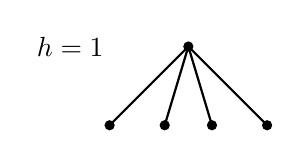
\begin{tikzpicture}
  \begin{scope}[every node/.style={thick,draw,circle,fill,scale=0.3}]
  \node (a) at (1,1) {};
  \node (b) at (0,0) {};
  \node (c) at (0.7,0) {};
  \node (d) at (1.3,0) {};
  \node (e) at (2,0) {};
  \end{scope}
  \begin{scope}[every edge/.style={draw=black,thick}]
  \path (a) edge (b);
  \path (a) edge (c);
  \path (a) edge (d);
  \path (a) edge (e);
  \end{scope}
  \node (l) at (-0.5,1) {$h = 1$};
  \end{tikzpicture}
\end{center}


\begin{center}
  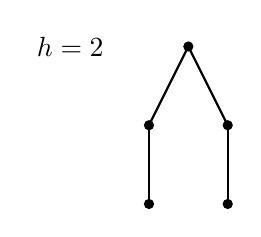
\begin{tikzpicture}
  \begin{scope}[every node/.style={thick,draw,circle,fill,scale=0.3}]
  \node (a) at (0.5,2) {};
  \node (b) at (0,1) {};
  \node (c) at (1,1) {};
  \node (d) at (0,0) {};
  \node (e) at (1,0) {};
  \end{scope}
  \begin{scope}[every edge/.style={draw=black,thick}]
  \path (a) edge (b);
  \path (a) edge (c);
  \path (b) edge (d);
  \path (c) edge (e);
  \end{scope}
  \node (l) at (-1,2) {$h = 2$};
  \end{tikzpicture}
  \hspace{0.4cm}
  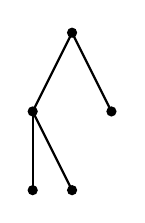
\begin{tikzpicture}
  \begin{scope}[every node/.style={thick,draw,circle,fill,scale=0.3}]
  \node (a) at (0.5,2) {};
  \node (b) at (0,1) {};
  \node (c) at (1,1) {};
  \node (d) at (0,0) {};
  \node (e) at (0.5,0) {};
  \end{scope}
  \begin{scope}[every edge/.style={draw=black,thick}]
  \path (a) edge (b);
  \path (a) edge (c);
  \path (b) edge (d);
  \path (b) edge (e);
  \end{scope}
  \end{tikzpicture}
  \hspace{0.4cm}
  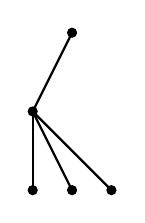
\begin{tikzpicture}
  \begin{scope}[every node/.style={thick,draw,circle,fill,scale=0.3}]
  \node (a) at (0.5,2) {};
  \node (b) at (0,1) {};
  \node (c) at (0,0) {};
  \node (d) at (0.5,0) {};
  \node (e) at (1,0) {};
  \end{scope}
  \begin{scope}[every edge/.style={draw=black,thick}]
  \path (a) edge (b);
  \path (b) edge (c);
  \path (b) edge (d);
  \path (b) edge (e);
  \end{scope}
  \end{tikzpicture}
  \hspace{0.4cm}
  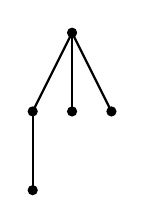
\begin{tikzpicture}
  \begin{scope}[every node/.style={thick,draw,circle,fill,scale=0.3}]
  \node (a) at (0.5,2) {};
  \node (b) at (0,1) {};
  \node (c) at (0.5,1) {};
  \node (d) at (1,1) {};
  \node (e) at (0,0) {};
  \end{scope}
  \begin{scope}[every edge/.style={draw=black,thick}]
  \path (a) edge (b);
  \path (a) edge (c);
  \path (a) edge (d);
  \path (b) edge (e);
  \end{scope}
  \end{tikzpicture}
\end{center}

\begin{center}
  \begin{tikzpicture}
  \begin{scope}[every node/.style={thick,draw,circle,fill,scale=0.3}]
  \node (a) at (0.5,3) {};
  \node (b) at (0,2) {};
  \node (c) at (1,2) {};
  \node (d) at (0,1) {};
  \node (e) at (0,0) {};
  \end{scope}
  \begin{scope}[every edge/.style={draw=black,thick}]
  \path (a) edge (b);
  \path (a) edge (c);
  \path (b) edge (d);
  \path (d) edge (e);
  \end{scope}
  \node (l) at (-1,3) {$h = 3$};
  \end{tikzpicture}
  \hspace{0.4cm}
  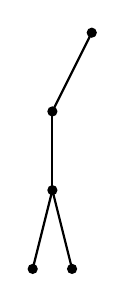
\begin{tikzpicture}
  \begin{scope}[every node/.style={thick,draw,circle,fill,scale=0.3}]
  \node (a) at (0.5,3) {};
  \node (b) at (0,2) {};
  \node (c) at (0,1) {};
  \node (d) at (-0.25,0) {};
  \node (e) at (0.25,0) {};
  \end{scope}
  \begin{scope}[every edge/.style={draw=black,thick}]
  \path (a) edge (b);
  \path (b) edge (c);
  \path (c) edge (d);
  \path (c) edge (e);
  \end{scope}
  \end{tikzpicture}
  \hspace{0.4cm}
  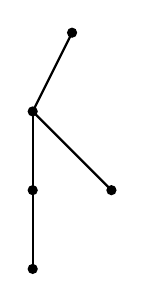
\begin{tikzpicture}
  \begin{scope}[every node/.style={thick,draw,circle,fill,scale=0.3}]
  \node (a) at (0.5,3) {};
  \node (b) at (0,2) {};
  \node (c) at (0,1) {};
  \node (d) at (1,1) {};
  \node (e) at (0,0) {};
  \end{scope}
  \begin{scope}[every edge/.style={draw=black,thick}]
  \path (a) edge (b);
  \path (b) edge (d);
  \path (b) edge (c);
  \path (c) edge (e);
  \end{scope}
  \end{tikzpicture}
\end{center}

\begin{center}
  \begin{tikzpicture}
  \begin{scope}[every node/.style={thick,draw,circle,fill,scale=0.3}]
  \node (a) at (0,4) {};
  \node (b) at (0,3) {};
  \node (c) at (0,2) {};
  \node (d) at (0,1) {};
  \node (e) at (0,0) {};
  \end{scope}
  \begin{scope}[every edge/.style={draw=black,thick}]
  \path (a) edge (b);
  \path (b) edge (c);
  \path (c) edge (d);
  \path (d) edge (e);
  \end{scope}
  \node (l) at (-1,3) {$h = 4$};
  \end{tikzpicture}
\end{center}

\end{solution}


\question
Construct two non-isomorphic rooted trees both having twelve vertices, six leaves, and height four~\cite{biggs02}.
\begin{solution}


\begin{center}
  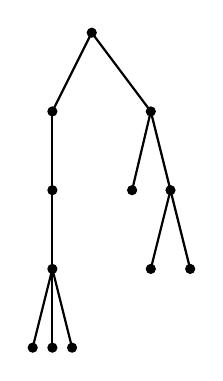
\begin{tikzpicture}
  \begin{scope}[every node/.style={thick,draw,circle,fill,scale=0.3}]
  \node (a) at (-0.5,4) {};
  \node (b) at (-1,3) {};
  \node (c) at (0.25,3) {};
  \node (d) at (-1,2) {};
  \node (e) at (0.0125,2) {};
  \node (f) at (0.5,2) {};
  \node (g) at (-1,1) {};
  \node (h) at (0.25,1) {};
  \node (i) at (0.75,1) {};
  \node (j) at (-1.25,0) {};
  \node (k) at (-1,0) {};
  \node (l) at (-0.75,0) {};
  \end{scope}
  \begin{scope}[every edge/.style={draw=black,thick}]
  \path (a) edge (b);
  \path (a) edge (c);
  \path (b) edge (d);
  \path (c) edge (e);
  \path (c) edge (f);
  \path (d) edge (g);
  \path (f) edge (h);
  \path (f) edge (i);
  \path (d) edge (g);
  \path (g) edge (j);
  \path (g) edge (k);
  \path (g) edge (l);
  \end{scope}
  \end{tikzpicture}
  \hspace{2cm}
  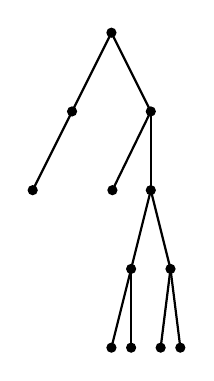
\begin{tikzpicture}
  \begin{scope}[every node/.style={thick,draw,circle,fill,scale=0.3}]
  \node (a) at (0,4) {};
  \node (b) at (-0.5,3) {};
  \node (c) at (0.5,3) {};
  \node (d) at (-1,2) {};
  \node (e) at (0.0125,2) {};
  \node (f) at (0.5,2) {};
  \node (g) at (0.25,1) {};
  \node (h) at (0.75,1) {};
  \node (i) at (0,0) {};
  \node (j) at (0.25,0) {};
  \node (k) at (0.625,0) {};
  \node (l) at (0.875,0) {};
  \end{scope}
  \begin{scope}[every edge/.style={draw=black,thick}]
  \path (a) edge (b);
  \path (a) edge (c);
  \path (b) edge (d);
  \path (c) edge (e);
  \path (c) edge (f);
  \path (f) edge (g);
  \path (f) edge (h);
  \path (g) edge (i);
  \path (g) edge (j);
  \path (h) edge (k);
  \path (h) edge (l);
  \end{scope}
  \end{tikzpicture}
\end{center}

\end{solution}

\question
Calculate the minimum height of a ternary rooted tree with ten leaves.
\begin{solution}


We have that $h \leq  \log_m l$.
Now, $\log_3 10 \approx 2.096$.
Since the minimum height must be a natural number, and this is a lower bound, we have that the minimum height is 3.
\end{solution}


\end{questions}